\chapter{Uso de bases de datos}
\section{PostgreSQL}
El proyecto usa distintas bases de datos segun el tipo de informacion que maneja cada servicio; este enfoque se conoce como persistencia poliglota. PostgreSQL se usa en Identity y Catalog. Identity guarda \texttt{users}; Catalog guarda \texttt{movie}, \texttt{genre}, \texttt{artist}, las tablas puente \texttt{movie\_genre} y \texttt{movie\_artist}, fuentes de video y subtitulos. Las relaciones N:M entre peliculas, generos y artistas se materializan mediante dichas tablas puente, y Flyway mantiene las versiones del esquema.

La Figura~\ref{fig:er_catalog_actualizado} presenta el diagrama ER actualizado del Catalog Service, con sus claves primarias, claves foraneas y relaciones fisicas.
\begin{figure}[H]
\centering
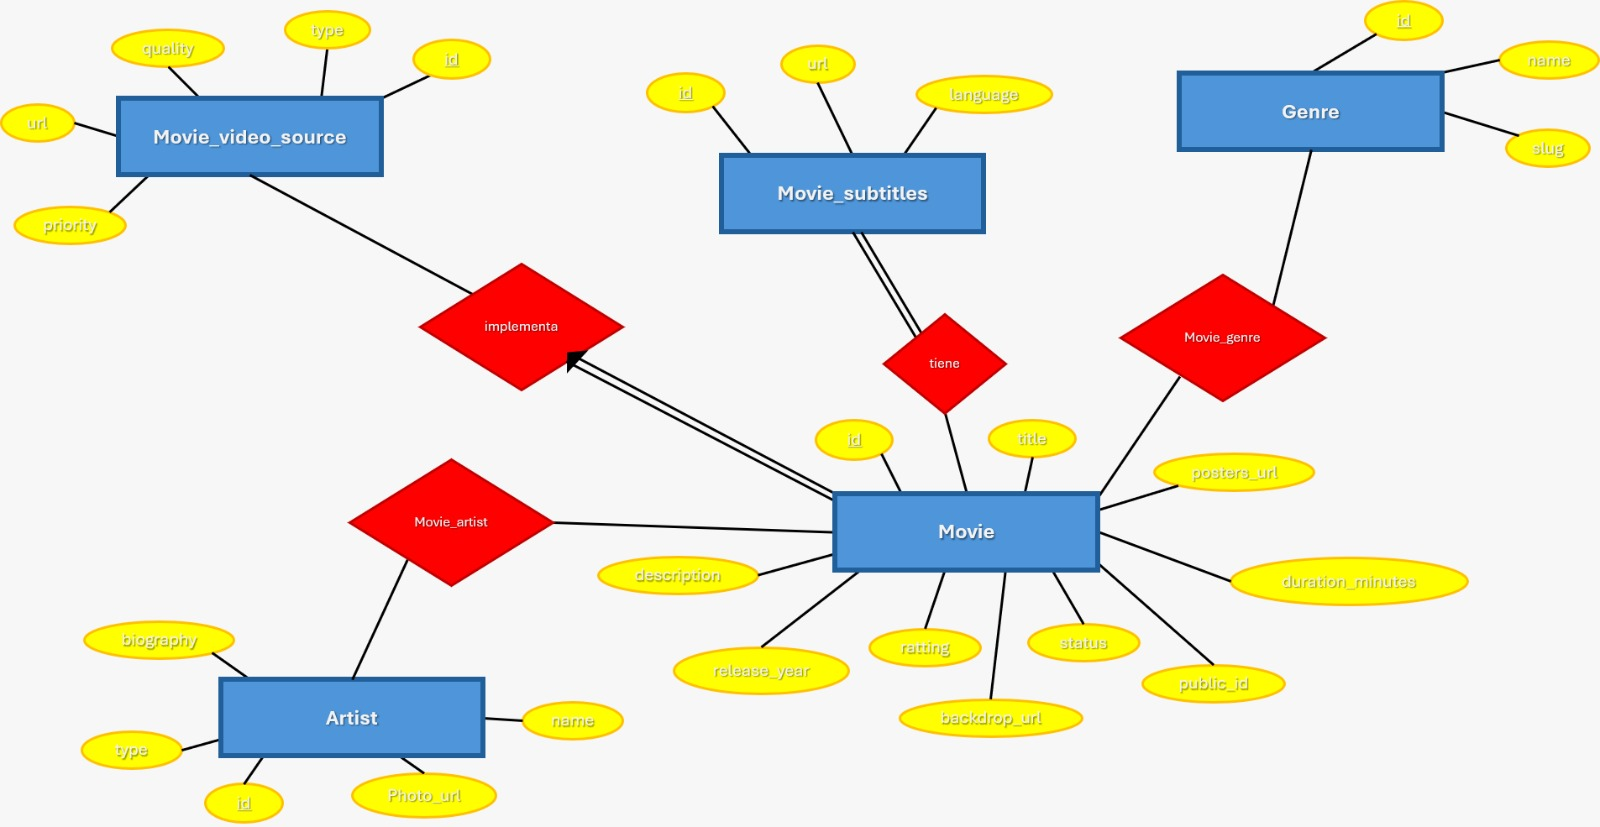
\includegraphics[width=\textwidth,height=.76\textheight,keepaspectratio]{../catalog.jpeg}
\caption{Diagrama ER actualizado del Catalog Service en PostgreSQL.}
\label{fig:er_catalog_actualizado}
\end{figure}

\section{MySQL}
Community usa MySQL para usuarios, clubes, membresias, salas y participantes. La tabla \texttt{memberships} materializa la relacion N:M entre usuarios y clubes. Las salas guardan el anfitrion y, si corresponde, el club; \texttt{watch\_participants} registra sus participantes. La Figura~\ref{fig:er_community_actualizado} presenta las claves primarias, claves foraneas y restricciones vigentes del Community Service. El campo \texttt{watch\_rooms.movie\_id} es una referencia logica hacia Catalog y no una clave foranea fisica entre MySQL y PostgreSQL.
\begin{figure}[H]
\centering
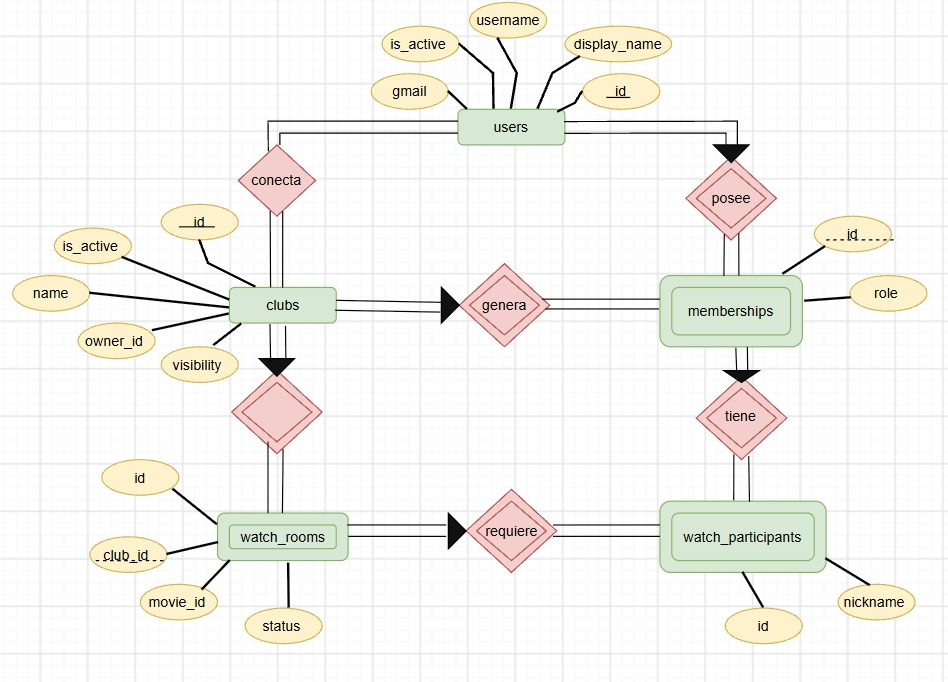
\includegraphics[width=\textwidth,height=.76\textheight,keepaspectratio]{../comunity.jpeg}
\caption{Diagrama ER actualizado del Community Service en MySQL.}
\label{fig:er_community_actualizado}
\end{figure}

\section{MongoDB}
Interaction usa MongoDB para \texttt{reviews}, \texttt{likes}, \texttt{watchlists} y \texttt{watch\_history}. Cada documento guarda la accion y una copia de los datos del usuario y de la pelicula. Los indices unicos de resenas y likes evitan que un usuario repita la misma accion sobre una pelicula.
\begin{figure}[H]\centering
\includegraphics[width=.92\textwidth]{figures/modelo-mongodb.pdf}\caption{Modelo documental MongoDB del Interaction Service}\label{fig:modelo_mongodb}\end{figure}
